\documentclass[]{article}
\usepackage{amsmath, amsfonts}
\usepackage{amssymb}
\usepackage{subcaption}
\usepackage{graphicx}
\usepackage{graphicx}
\usepackage{dblfloatfix}
\usepackage{color}
\definecolor{lightgray}{gray}{0.5}
\setlength{\parindent}{0pt}

%opening
\title{Homework 1: Extended Yale Faces B Database – Eigenfaces}
\author{Evan Ko}
\pagenumbering{arabic}

\begin{document}

	\maketitle

\begin{abstract}
This paper presents the versatility of the singular value decomposition and principal component analysis. Singular value decomposition (SVD) is one of the most important and useful factorizations in linear algebra. Using the Yale Faces Database we will explore how a singular value decomposition(svd) analysis can reconstruct a face.In this paper I will explore the difference a cropped versus an uncropped image has on the svd's ability to reconstruct an image.
\end{abstract}

\section{Introduction and Overview}
Every person has a face but we don't all look alike. Every face has its unique defining feature. Given a database of pictures can you from the generate
\section{Theoretical Background }
The singular value decomposition drives this whole report.The SVD is a factorization of matrix into a number of constitutitve components all of which have a specific meaning in applications. SVD breaks the matrix A into three components U $\Sigma$ and V. If $A\in \mathbb{R}^{mxn}$ then $U\in\mathbb{C}^{mxm},V\in\mathbb{C}^{nxn}$, and $\Sigma \in \mathbb{R}^{mxn}$. U and V are unitary matrices and $\Sigma$ is a diagonal matrix where the singular values are ordered from largest to smallest so that $\sigma_1\geq\sigma_2\geq\dots\geq\sigma_p\geq0$ where p = min(m,n)\\
The U,$\Sigma$ and V matrices can be interpreted as a change of basis to the A matrix. V applies an unitary transformation or a rotation, and $\Sigma$ scales how much of the matrix is stretched, and U is another transformation.   
\section{ Algorithm Implementation and Development }
\begin{enumerate}
	\item \textbf{Constructing data matrix}\\
	To begin the analysis, a data matrix needs to be formed. After reading in the images from the database, each image was reshaped using the MATLAB command \textbf{reshape} into a 1 column vector where all the rows are a pixel from the image. The data matrix is thus all the column image vectors in one matrix. The data matrix is also mean centered by subtracting the row mean from the 
	\item \textbf{Compute the SVD reconstruct matrix}\\
	Using the MATLAB command \textbf{svd} the u,s,and v matrix is computed
	\item \textbf{Check the singular values}\\
	We plot the percent correlation of singular value by first getting the diagonal of the s matrix and plotting the diagonals of s/sum(diagonals of s). We plot the normalized diagonals to see which norms are relevant.
	\item \textbf{reconstruction of faces}\\
	We explore the effect of using more or less "energy" to reconstruct a an image using the svd.We reconstructed the data matrix using A = $U*\Sigma*V^T$.The amount of modes we used was translated as how much of the column space of each matrix, u,s,v, were used to recreate the data matrix. For instance 4 modes would be A4 = $U(:,1:4)*\Sigma(1:4,1:4)*V(:,1:4).'$ In the uncropped images we used 4,50,75,rank of matrix, and all modes to reconstruct the images. In the cropped images we used 4,50,500,rank of matrix, and all modes to reconstruct the images. 
	\item \textbf{viewing of eigenfaces}\\
	Finally we checked out the eigenfaces and plotted the first 16 by first reshaping the column into a matrix and viewing by the MATLAB command \textbf{pcolor}.  
\end{enumerate}

\section{Computational Results}
\subsection{Uncropped images}
We will start with the uncropped image set. After computing the svd of the data set we first look at the singular values and the percent correlation that the singular values hold. 
\begin{figure}[!htbp]
	\begin{subfigure}{\linewidth}
		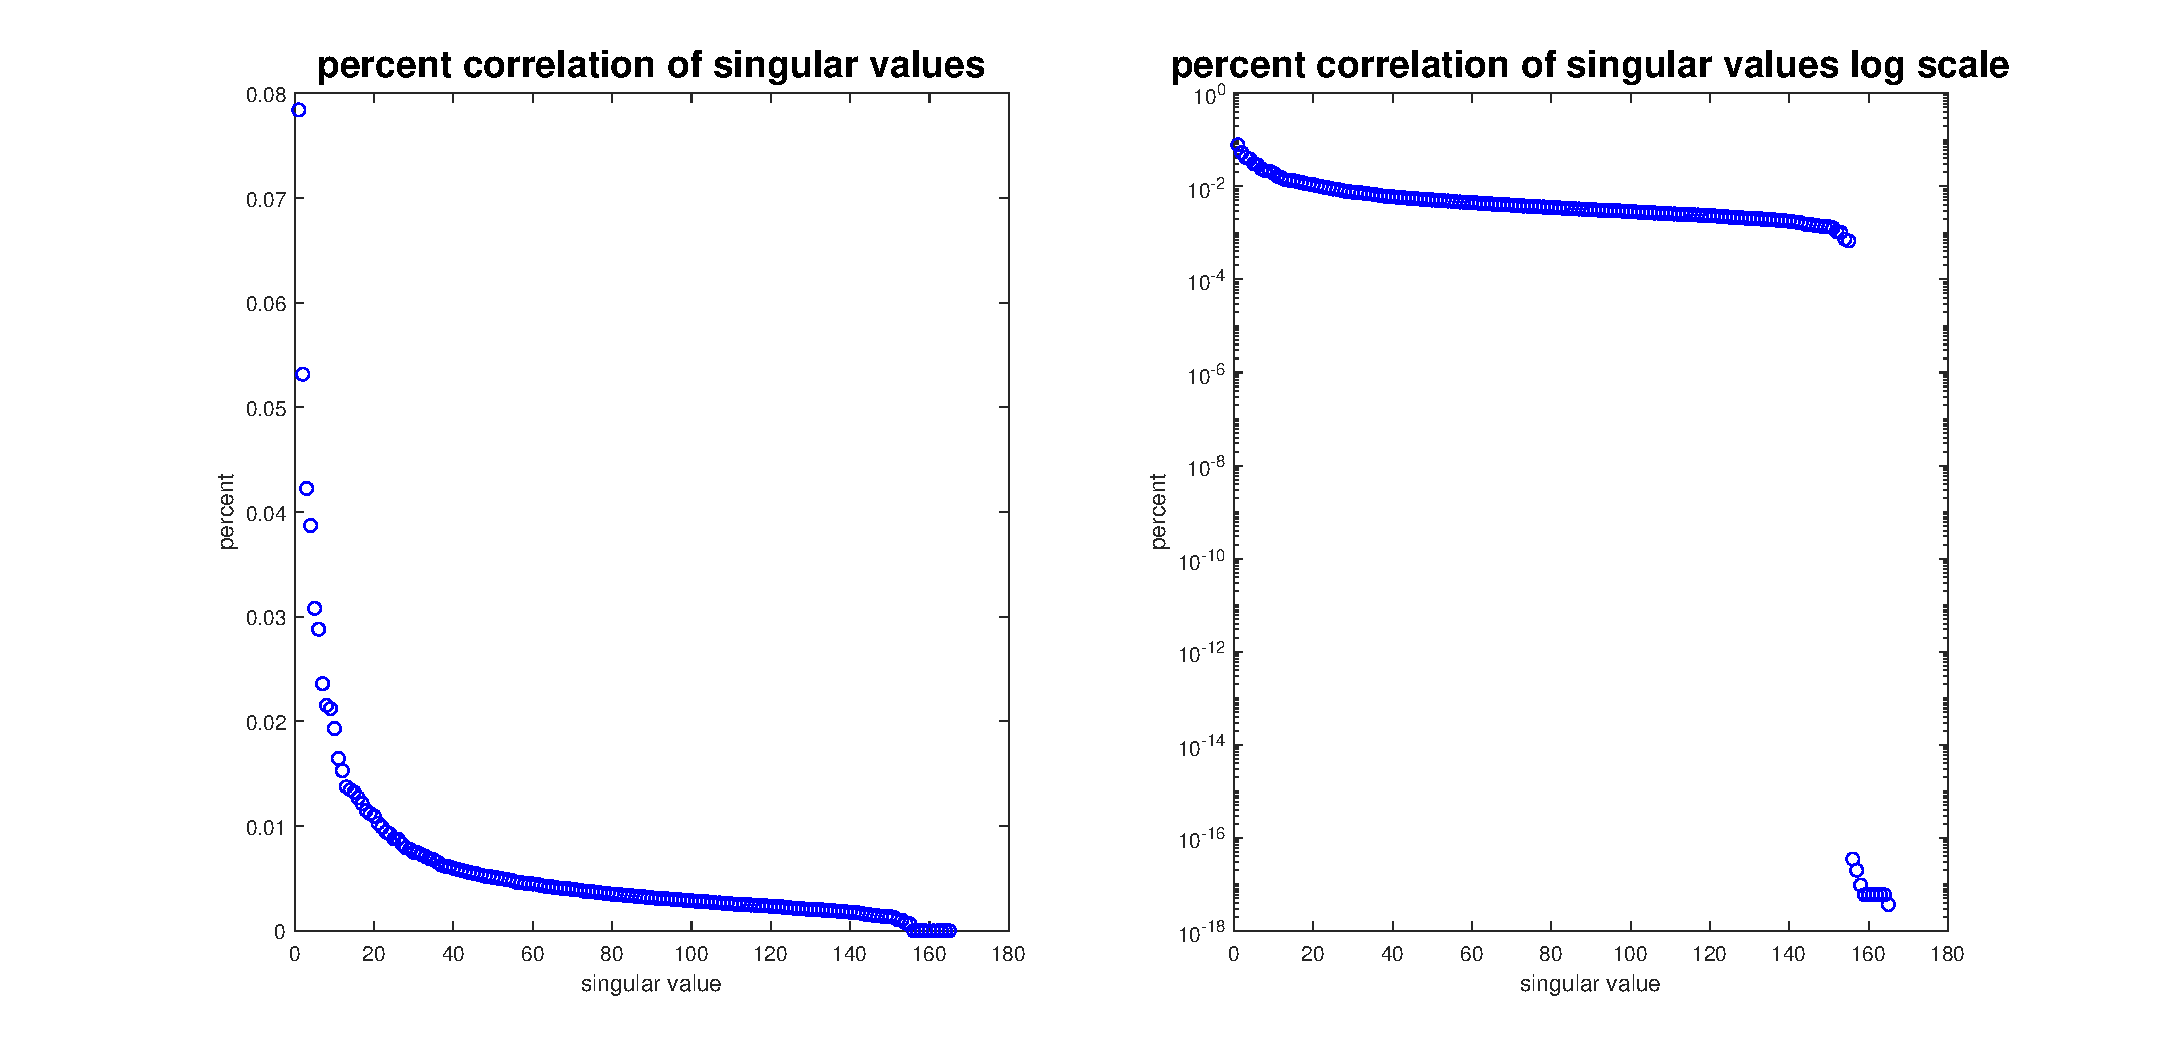
\includegraphics [width=4in]{ucPercent.eps}
		\caption{percent correlation of singular values}
	\end{subfigure}	
	\begin{subfigure}{\linewidth}
		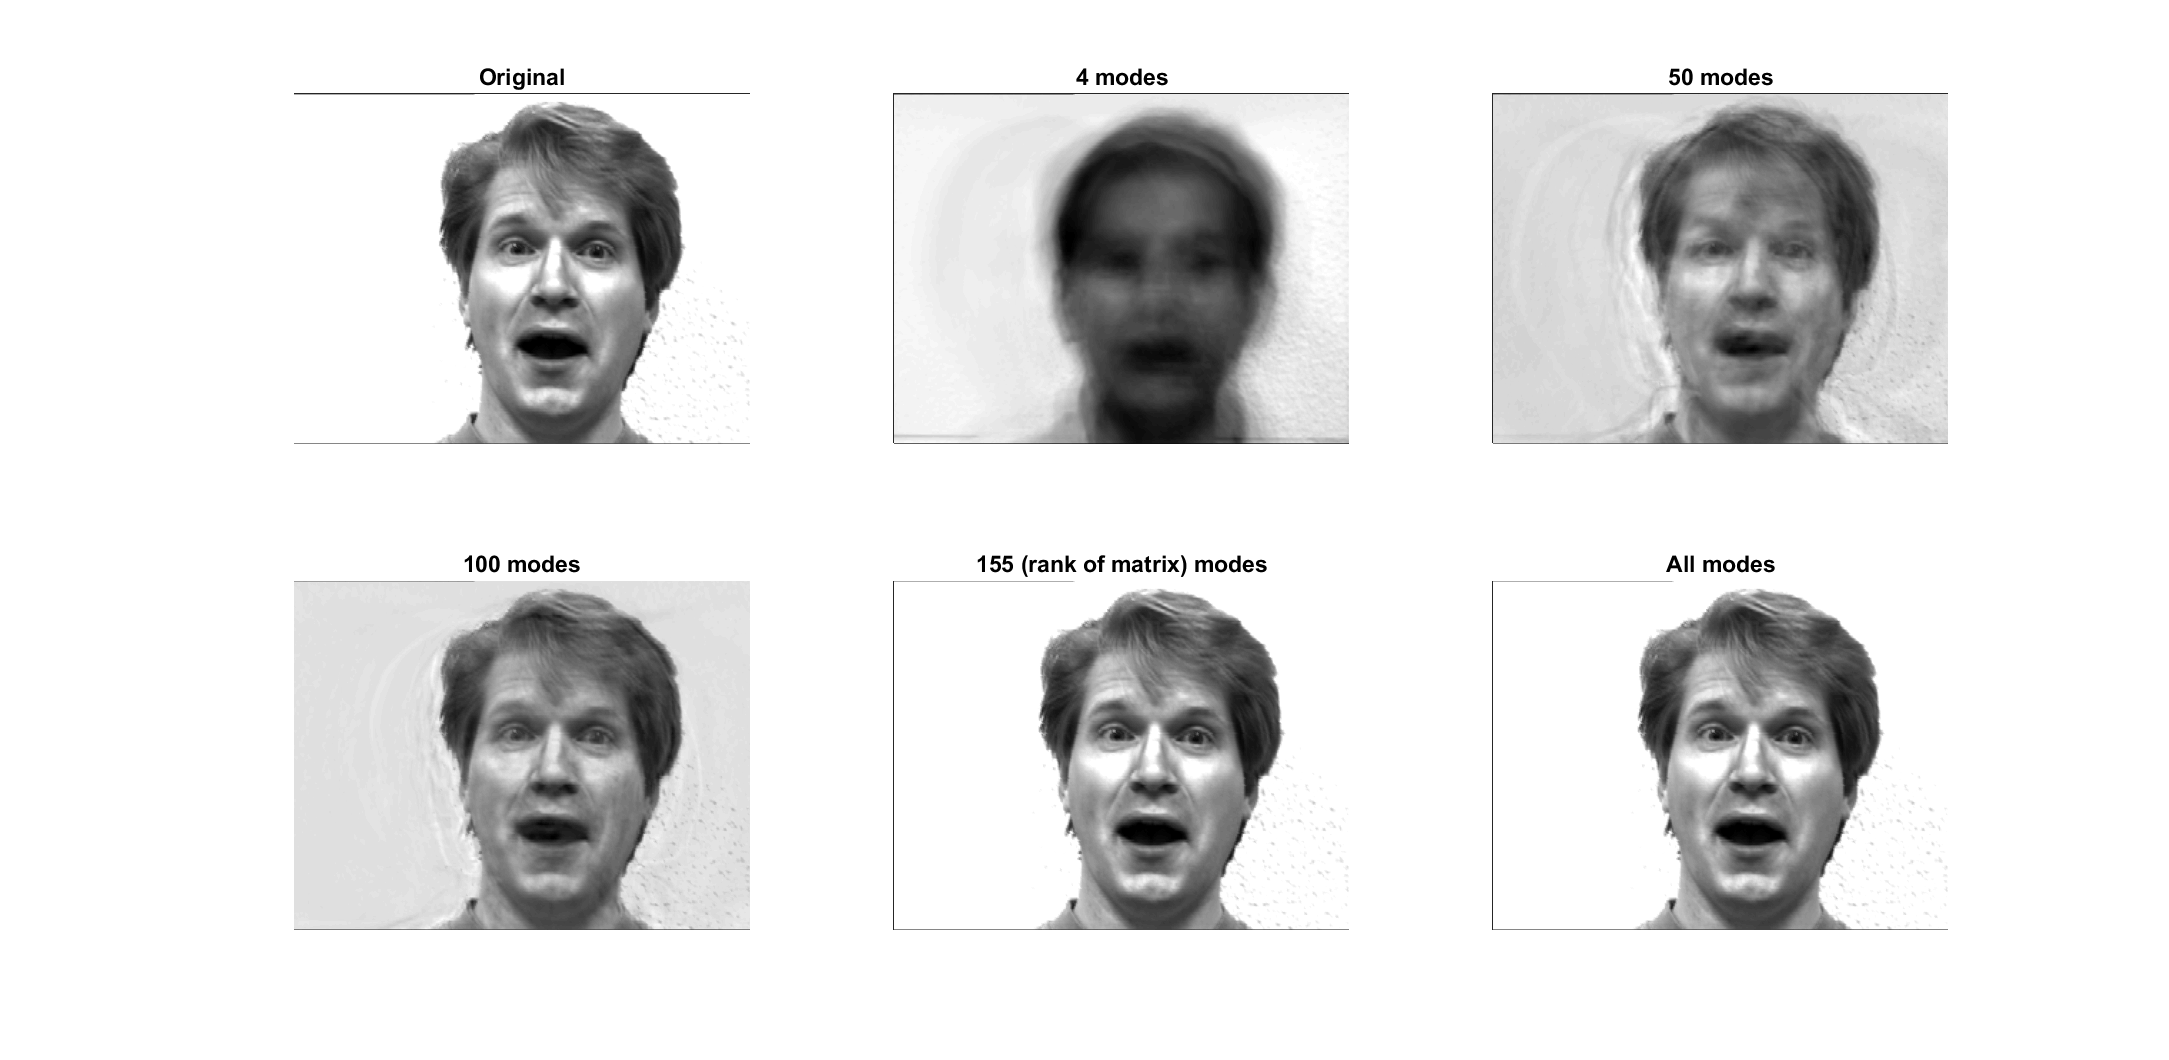
\includegraphics [width=4in]{ucReconstruction.eps}
		\caption{facial reconstruction using different modes}
	\end{subfigure}
	\begin{subfigure}{\linewidth}
		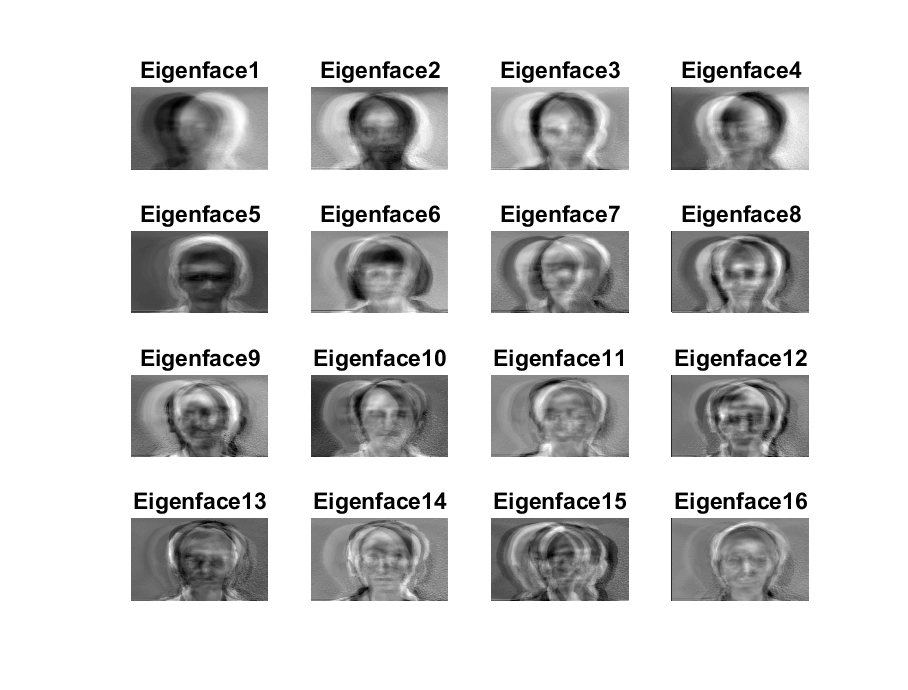
\includegraphics [width=4in]{ucEigenface.eps}
		\caption{the first 16 eigenfaces}
	\end{subfigure}
	\caption{all plots for uncropped image}
\end{figure}
From figure 1.a we see that it looks like most of the values are non-zero. The plot on the right which is on a log base shows almost all the values are non-zero. In fact when we compute the rank of the s matrix we get 155. Thus 155/165 = 0.94 or 94\% is non-zero meaning that 155 modes were needed to fully reconstruct the data matrix. \\
In figure 1.b we see the difference using more modes has on the overall clearness of the images. Here in figure 2 we reconstruct image 10 from the image set.
As you can see using 4 modes to reconstruct the image does not yield a good reconstruction of the image. At 50 modes we see that the face looks the same but there are some other "heads" in the picture and the background is off. It isn't until we use the rank of the matrix, 155 modes that the original picture is reconstructed. The addition of all the modes doesn't have any affect on the overall quality of the image.\\
In figure 1.c we see that each of the modes came from the eigenfaces from the U matrix. We see that by plotting the first 16 eigenfaces, that the combination of the first 4 get close to the face of the 4 mode image, but many more would be needed to get back the original image.\\
We see that since every face isn't in the same position there are many faces that make up the first 16 eigenfaces.
\subsection{Cropped image}
We continue with the cropped image set. After computing the svd of the data set we first look at the singular values and the percent correlation that the singular values hold.
\begin{figure}[htbp]
	\begin{subfigure}{\linewidth}
		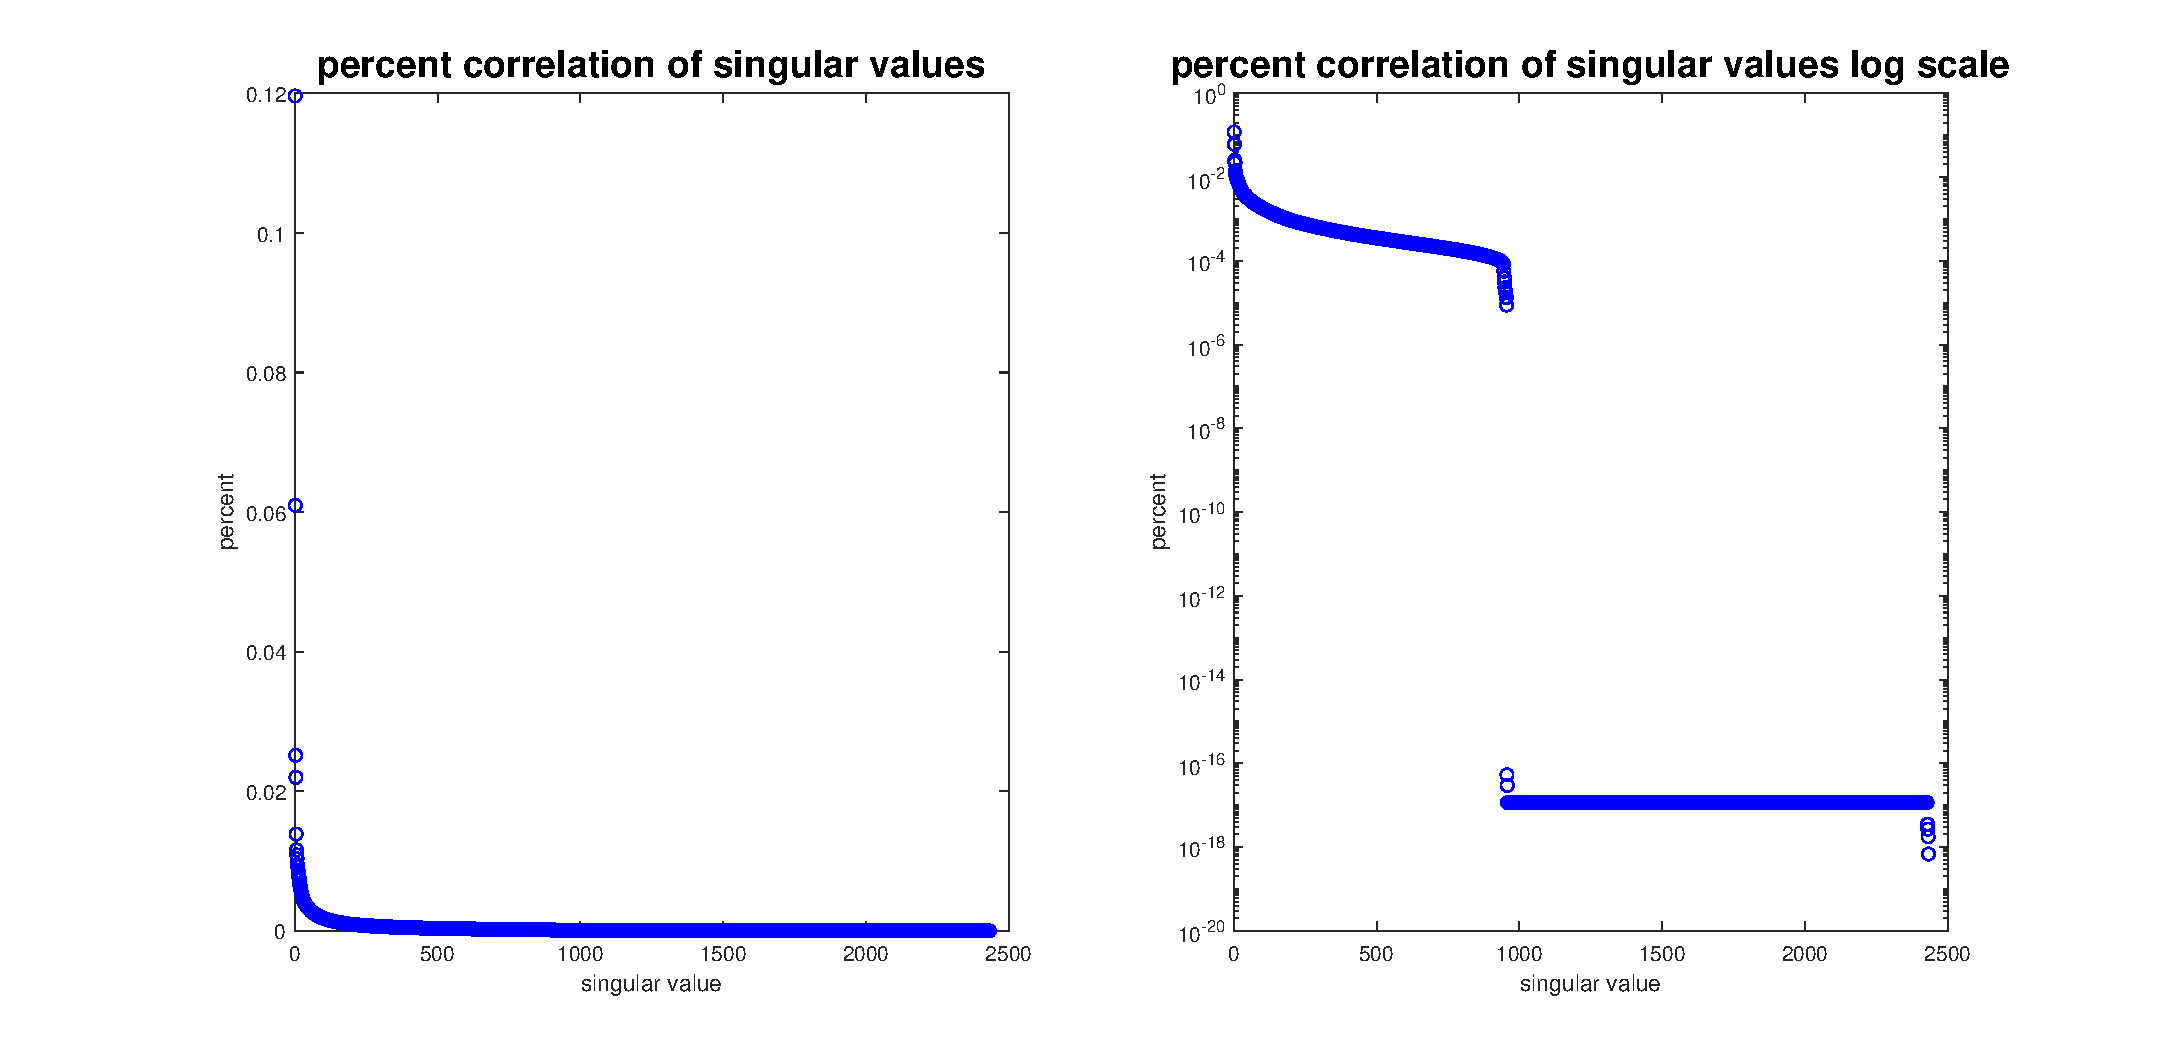
\includegraphics [width=4in]{cPercent.eps}
		\caption{percent correlation of singular values}
	\end{subfigure}	
	\begin{subfigure}{\linewidth}
		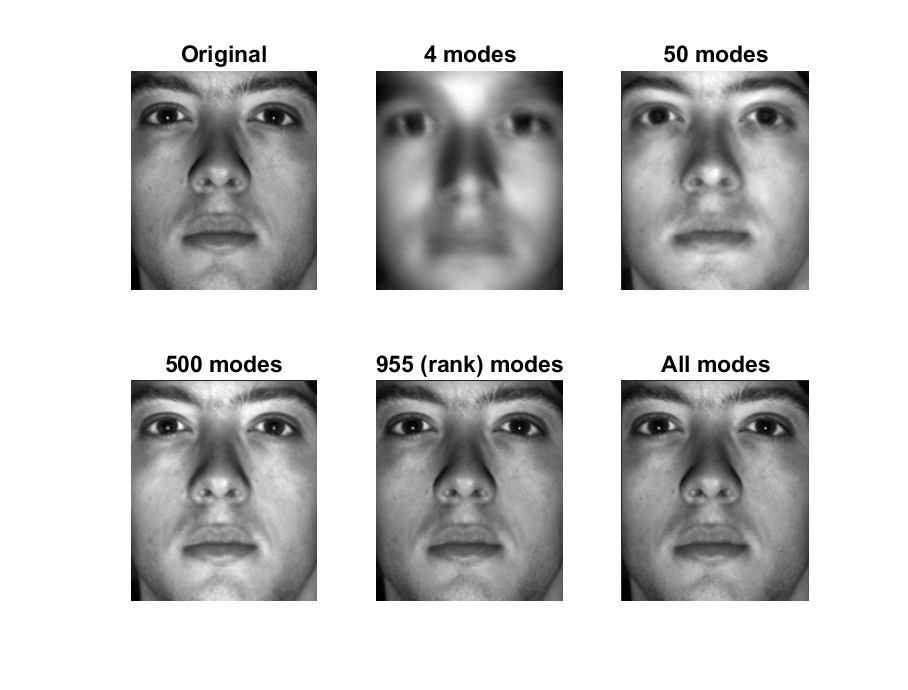
\includegraphics [width=4in]{cReconstruction.eps}
		\caption{facial reconstruction using different modes}
	\end{subfigure}
	\begin{subfigure}{\linewidth}
		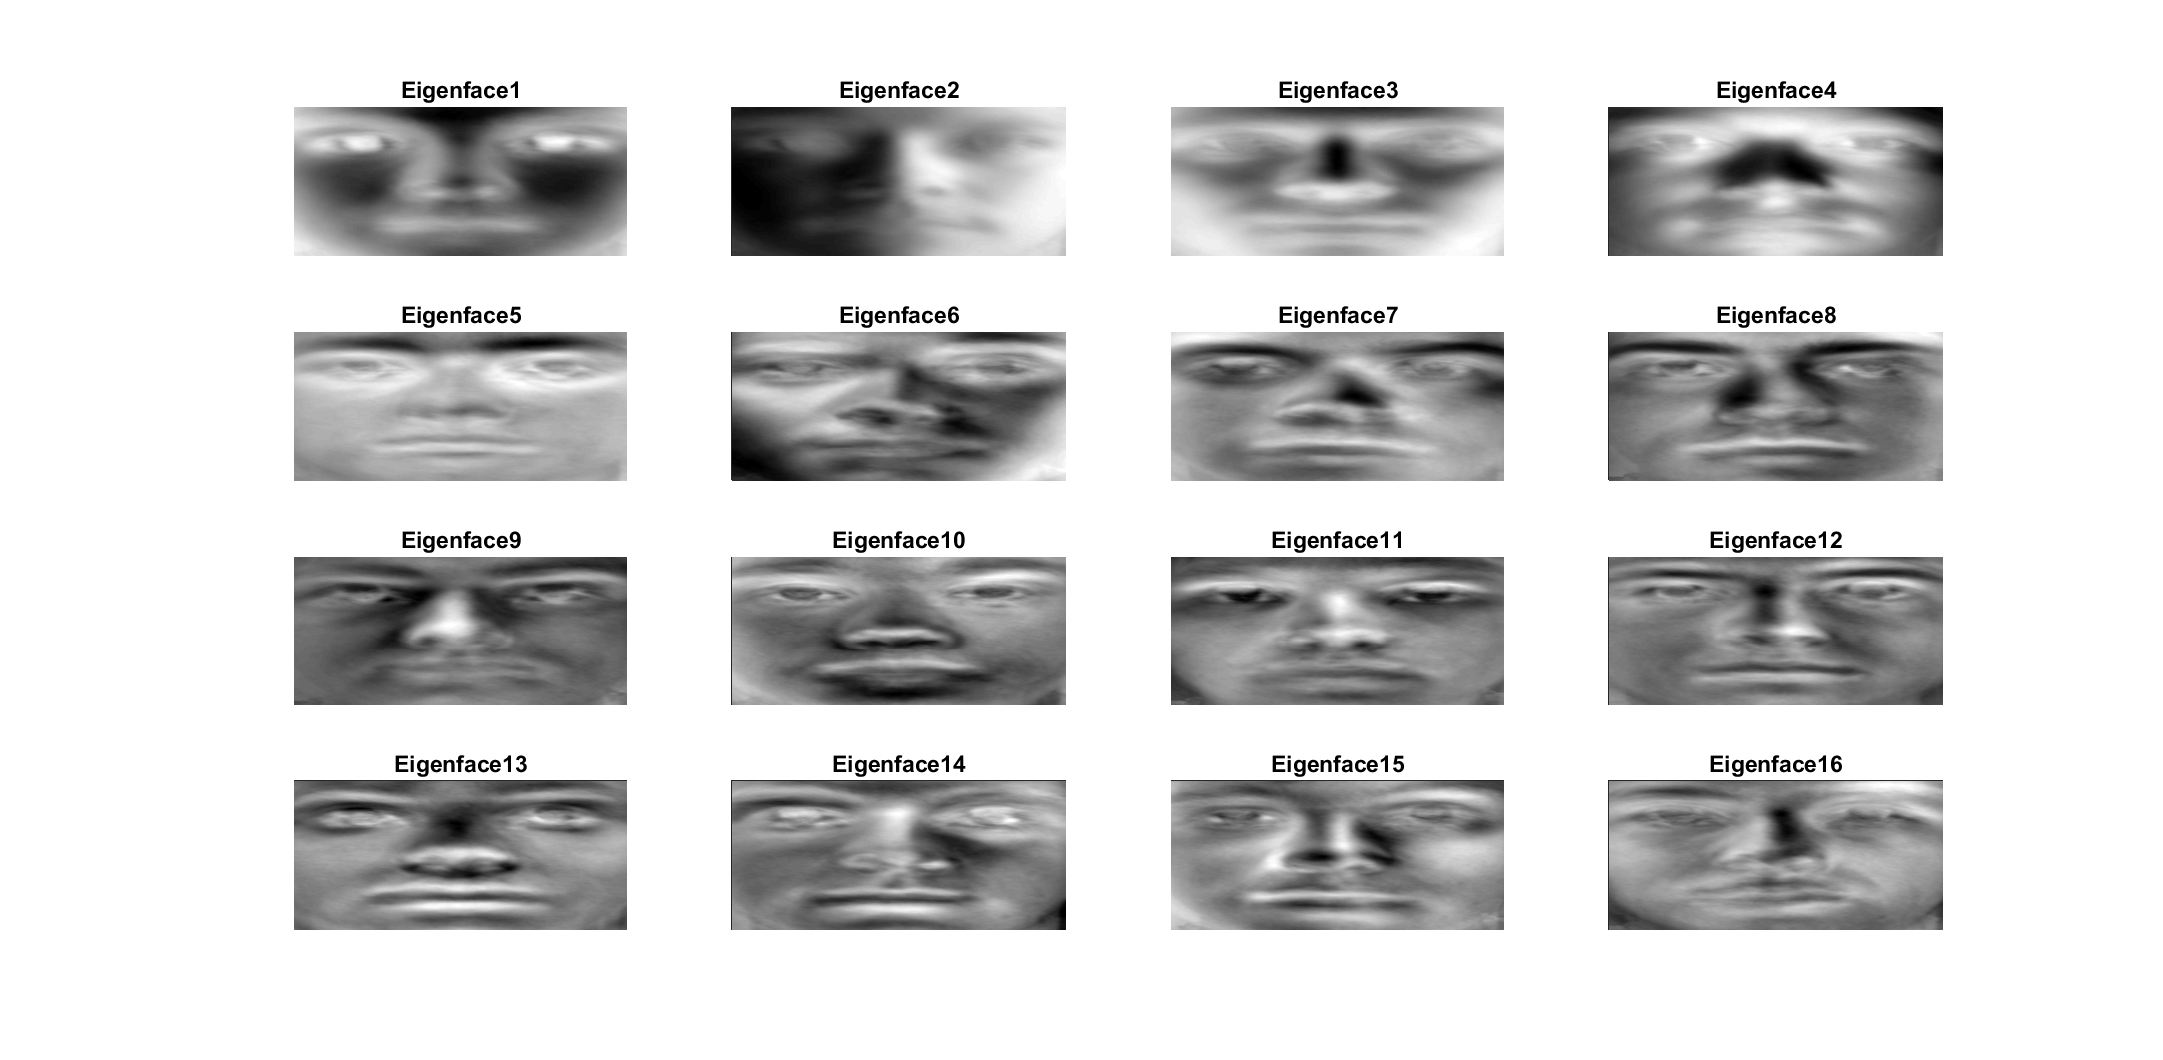
\includegraphics [width=4in]{cEigenface.eps}
		\caption{the first 16 eigenfaces}
	\end{subfigure}
	\caption{all plots for cropped image}
\end{figure}
In figure 2.a we see that some of the points are non-zero. It is hard to tell on the left plot, so the plot was plotted on a log scale. The plot on the right shows about half the values are non-zero. In fact when we compute the rank of the s matrix we get 955. Thus 955/2432 = 0.393 or 39\% is non-zero meaning that 955 modes were needed to fully reconstruct the data matrix. \\
From figure 2.b we can extrapolate using more modes has an affect on the overall clearness of the images. Here in figure 5 we reconstruct image 115 from the image set.\\
As you can see using 4 modes to reconstruct the image does not yield a good reconstruction of the image. At 50 modes we see that the face looks almost the same but the mouth is not correct and the color is wrong. At 500 modes the mouth is correct but the color is still wrong. It isn't until using 955 modes that the original image was reconstructed. Using all the modes did not not have any affect on the overall clearness of the image.\\
In figure 2.c we see each of the modes that came from the eigenfaces from the U matrix. We see that by plotting the first 16 eigenfaces, that the combination of the first 4 get close to the face of the 4 mode image, but many more would be needed to get back the original image.
We see that the faces are only one face. The faces do not have many defining features but it is just one face in each image
\section{Summary and Conclusions}
There were many similarities and difference between the cropped and uncropped images reconstructed. The cropped image set had all the faces in the same position taking the entire image while the uncropped image had the faces in different positions and a background in the images. The difference between the image sets meant that only 39\% of the modes were needed to reconstruct the cropped image but 94\% of the modes were needed to reconstruct the uncropped image. The difference of almost 3 times the amount of modes needed to get a good reconstruction of an uncropped image meant that the addition of 50 modes did not have a great affect on the overall picture. Using SVD on the data matrix from both image sets, we were able to reconstruct the original image.Performing SVD on the data matrix gives us the ability to reconstruct any image from the original image set. 
\section{ MATLAB functions used and brief implementation explanation }
svd: Used to do svd analysis on the image set\\
dir: Used to find the images\\
imread: read in the image files\\
pcolor: show the image from a double matrix\\
reshape: reshape the matrix into another dimensional matrix
\section{MATLAB codes }
\subsection{uncropped script}
\begin{verbatim}
clear global; close all; clc
imageList = dir('./yalefaces_uncropped/yalefaces');
matrix = ones(243*320,length(imageList)-2);
for i = 3:length(imageList)
[X,map] = imread(strcat('./yalefaces_uncropped/yalefaces/',imageList(i).name));
rx = reshape(double(X),243*320,1);
matrix(:,i-2) = rx;
end
%center mean the matrix
avgM = mean(matrix,2);
matrix = matrix - avgM;
%% calculate the svd of the matrix
[u,s,v] = svd(matrix,'econ');
%% plot the percent correlation of singular values
figure(1)
subplot(1,2,1)
plot(diag(s)/sum(diag(s)),'bo'), 
title('percent correlation of singular values','fontsize',18),
xlabel('singular value'),ylabel('percent')
subplot(1,2,2)
semilogy(diag(s)/sum(diag(s)),'bo'),
title('percent correlation of singular values log scale','fontsize',18)
,xlabel('singular value'),ylabel('percent')
rankM = rank(s);
%% reconstruct image from svd using different percentage of energy 
imageIndex = 10;

%remake the first image
A1 = reshape(matrix(:,imageIndex)+avgM,243,320);
figure(2)
subplot(2,3,1),pcolor(flipud(A1)), shading interp,colormap(gray),
set(gca,'Xtick',[],'Ytick',[]),
title('Original')

%using 4 modes
rank4 = u(:,1:4)*s(1:4,1:4)*v(:,1:4).';
rrank4 = reshape(rank4(:,imageIndex)+avgM,243,320);
subplot(2,3,2),pcolor(flipud(rrank4)), shading interp,colormap(gray),
set(gca,'Xtick',[],'Ytick',[]),
title('4 modes')

%using 50 modes
rank50 = u(:,1:50)*s(1:50,1:50)*v(:,1:50).';
rrank50 = reshape(rank50(:,imageIndex)+avgM,243,320);
subplot(2,3,3),pcolor(flipud(rrank50)), shading interp,colormap(gray),
set(gca,'Xtick',[],'Ytick',[]),
title('50 modes')

%using 100 modes
rank100 = u(:,1:100)*s(1:100,1:100)*v(:,1:100).';
rrank100 = reshape(rank100(:,imageIndex)+avgM,243,320);
subplot(2,3,4),pcolor(flipud(rrank100)), shading interp,colormap(gray),
set(gca,'Xtick',[],'Ytick',[]),
title('100 modes')

%using 155 modes or rank of matrix
rankR = u(:,1:rankM)*s(1:rankM,1:rankM)*v(:,1:rankM).';
rrankR = reshape(rankR(:,imageIndex)+avgM,243,320);
subplot(2,3,5),pcolor(flipud(rrankR)), shading interp,colormap(gray),
set(gca,'Xtick',[],'Ytick',[]),
title('155 (rank of matrix) modes')

%using all modes
rankTotal = u*s*v.';
rrankTotal = reshape(rankTotal(:,imageIndex)+avgM,243,320);
subplot(2,3,6),pcolor(flipud(rrankTotal)), shading interp,colormap(gray),
set(gca,'Xtick',[],'Ytick',[]),
title('All modes')

%% check out the eigenfaces
figure(3)
for k = 1:16
ee = reshape(u(:,k),243,320);
subplot(4,4,k)
pcolor(flipud(ee)),shading interp,colormap(gray),set(gca,'Xtick',[],'Ytick',[]),
title(strcat('Eigenface ',num2str(k)))
end
\end{verbatim}
\subsection{cropped script}
\begin{verbatim}
clear globals; close all; clc
matrix = ones(192*168,2414); 
folderList = dir('./CroppedYale');
for i = 3:length(folderList)
imglist = dir(strcat('./CroppedYale/',folderList(i).name));
if ~isempty(imglist)
for j = 3:le+ngth(imglist)
imglist(j).name;
[X,map] = imread(strcat('./CroppedYale/',folderList(i).name,'/',imglist(j).name));
dX = double(X);
rX = reshape(dX,192*168,1);
matrix(:,(i-2)*(j-2)) = rX;
end
end
end

avgM = mean(matrix,2);
matrix = matrix - avgM;

[u,s,v] = svd(matrix,'econ');
%%
figure(1)
subplot(1,2,1)
plot(diag(s)/sum(diag(s)),'bo'), 
title('percent correlation of singular values','fontsize',18),
xlabel('singular value'),ylabel('percent')
subplot(1,2,2)
semilogy(diag(s)/sum(diag(s)),'bo'),
title('percent correlation of singular values log scale','fontsize',18),
xlabel('singular value'),ylabel('percent')
rankM = rank(s);

%%
imageIndex = 115;

%remake the first image
figure(2)
A1 = reshape(matrix(:,imageIndex)+avgM,192,168);
subplot(2,3,1),pcolor(flipud(A1)), 
shading interp,colormap(gray),set(gca,'Xtick',[],'Ytick',[]),title('Original')

%using 4 modes
rank4 = u(:,1:4)*s(1:4,1:4)*v(:,1:4).';
rrank4 = reshape(rank4(:,imageIndex)+avgM,192,168);
subplot(2,3,2),pcolor(flipud(rrank4)), 
shading interp,colormap(gray),set(gca,'Xtick',[],'Ytick',[]),title('4 modes')

%using 50 modes
rank50 = u(:,1:50)*s(1:50,1:50)*v(:,1:50).';
rrank50 = reshape(rank50(:,imageIndex)+avgM,192,168);
subplot(2,3,3),pcolor(flipud(rrank50)), 
shading interp,colormap(gray),set(gca,'Xtick',[],'Ytick',[]),title('50 modes')

%using 500 modes
rank500 = u(:,1:500)*s(1:500,1:500)*v(:,1:500).';
rrank500 = reshape(rank500(:,imageIndex)+avgM,192,168);
subplot(2,3,4),pcolor(flipud(rrank500)), 
shading interp,colormap(gray),set(gca,'Xtick',[],'Ytick',[]),title('500 modes')

%using 955 modes
rankR = u(:,1:rankM)*s(1:rankM,1:rankM)*v(:,1:rankM).';
rrankR = reshape(rankR(:,imageIndex)+avgM,192,168);
subplot(2,3,5),pcolor(flipud(rrankR)), 
shading interp,colormap(gray),set(gca,'Xtick',[],'Ytick',[]),title('955 (rank) modes')

%using all modes
rankTotal = u*s*v.';
rrankTotal = reshape(rankTotal(:,imageIndex)+avgM,192,168);
subplot(2,3,6),pcolor(flipud(rrankTotal)), 
shading interp,colormap(gray),set(gca,'Xtick',[],'Ytick',[]),title('All modes')


%%
%try to model the eigenfaces
figure(3)
for k = 1:16
ee = reshape(u(:,k),192,168);
subplot(4,4,k)
pcolor(flipud(ee)),shading interp,colormap(gray),
set(gca,'Xtick',[],'Ytick',[]),title(strcat('Eigenface  ',num2str(k)))
end
\end{verbatim}




\end{document}
